\chapter{Irodalom}
\pagestyle{headings}

Ebben a fejezetben a szakdolgozatom hátteréül szolgáló ismeretanyagot tekintem át. A fejezet két jól elkülönülő részből áll. Az első alfejezetben a pásztázó elektrokémiai mikroszkópia irodalmát mutatom be. A teljességre nem törekedve ismertetem kifejlesztésének főbb állomásait, a módszer működési elvét, fejlődését és felhasználási területeit. A fejezet második alfejezetében a pásztázó elektrokémiai mikroszkóp általam vizsgált új alkalmazási módjának példájául szolgáló Belouszov-Zsabotyinkszkij oszcilláló reakcióval foglalkozok. 

\section{Pásztázó elektrokémiai mikroszkópia}
\subsection{Története}
\subsection{Működése}
\subsubsection{Potenciometria}
Egy elektroanalitikai eljárás során a mérőcellába lévő mintába merülő elektródokat használunk, mely a vizsgálat típusától függően 2-4 lehet. Az elektródokat funkciójuk szerint különítjük el, lehet indikátorelektród (munkaelektród), referenciaelektród (vonatkozási elektród) illetve segédelektród. Indikátor elektródként elsőfajú fémelektródokat, vagy 1-1 ionra szelektív elektródokat használhatunk, melyek lehetnek ionszelektív-, gáz-, redoxi- vagy enzimelektródok. Referenciaelektródnak másodfajú elektródokat alkalmazunk a méréseink során, amik egy fémből, a fém sójából és a só anionjának nagy koncentrációjú oldatából készül.
Az elektroanalitikai vizsgálatok közül a leggyakrabban alkalmazott módszer a potenciometria [16]. A potenciometria során az elektrolitoldatba merített elektródok felületén kialakuló potenciál különbséget mérjük. Az elektrokémiai cella (jelen esetben galváncella) egy indikátor- és egy referenciaelektródból áll, e két félcella között mérjük a potenciálkülönbséget, miközben áram nem folyik át a cellán. Az elektródpotenciál és az elektród aktív komponens közötti összefüggést a Nernst-egyenlet adja meg: 
\begin{equation}
E = E_\text{0} + \frac{RT}{zF} \ln a
\end{equation}

ahol $E$ a cellapotenciál, $E_\text{0}$ a rendszer standard potenciálja, $R$ a gázállandó, $T$ a termodinamikai hőmérséklet, $z$ az elektródfolyamat elektronszám-változása,az $F$ a Faraday-állandó, $a$ az elektródaktív komponens aktivitása.

Az aktivitás (a) és a koncentráció kapcsolatát az a=fc összefüggés adja meg, ahol f az aktivitási koefficiens. Híg oldatok esetén feltételezzük, hogy $f=1$, tehát $a=c$. A töményebb oldatok esetén, amikor $f\neq 1$, abban az esetben az aktivitási koefficiens állandó értéken tartásával és ily módon végzett kalibrációval kapunk analitikai információt. A gyakorlatban a fent említett Nernst-egyenletet koncentrációra felírva (c) és tizes alapú logaritmus formájában használjuk:
\begin{equation}
E= E_\text{0} + \frac{0.059}{z} \ln c
\end{equation}
Az elektródpotenciálból, tehát az azt létrehozó elektródaktív komponens koncentrációja kiszámítható. Egy elektród felületén kialakuló feszültséget közvetlenül nem lehet mérni, ezért a vizsgálat során a keresendő komponens koncentrációja által generált potenciált mérjük az indikátorelektródon az állandó pontenciálú referenciaelektróddal szemben. Ezt az állandó potenciált a referenciaelektródon úgy tudjuk biztosítani, hogy a belső töltőoldatát állandó értéken tartjuk, ezt a referenciaelektród elválasztásával tudjuk elérni. A két elektród kapcsolódását sóhíd használatával valósítjuk meg egy folyadék-folyadék határfelület jön létre, ami szinte potenciálkülönbséget eredményez, ezt diffúziós potenciálnak nevezzük. Ez a diffúziós potenciál a mérések során mindig fennáll, ugyanis nem tudjuk teljes mértékben megszűntetni. Ennek kiküszöbölésére a két félcellát egy sóhíddal kötik össze, a sóhídban található só oldatot, olyan anyagból készítik, ami anionjának és kationjának mozgékonysága körülbelül megegyezik. [16]

%\begin{table}[]
%\centering
%\caption{My caption}
%\label{my-label}
%\begin{tabular}{llll}
%\multicolumn{4}{l}{Ionok mozgékonysága vizes oldatban, 25 \textdegree C hőmérsékleten} \\
%H$^\{+}$       & 36,3*10-8      & OH$^\-$        & 20,5 $\times$ 10$^{-8}$     \\
%K$^\{+}$       & 7,62*10-8      & SO_\text{4} ^\2-     & 8,27 $\times$ 10$^{-8}$     \\
%Na$^\{+}$      & 5,19*10-8      & Cl$^\-$        & 7,91*10-8     \\
%Li$^\+$      & 4,01*10-8      & NO_\text{3} ^\-      & 7,4*10-8     
%\end{tabular}
%\end{table}

A táblázatban látható, hogy a kálium-,klorid- és a nitrátion mozgékonysága nagyjából megegyezik, ezért például használhatunk KCl és KNO3 oldatot.
A fent említett oldatok esetén a diffúzió során a kation és az anion közel azonos sebességgel halad, így nem lesz töltésfeldúsulás. Fontos még, hogy a sóhídat képző oldat koncentrációja a vizsgálandó oldat és a referenciaelektród töltőoldatánál nagyobb legyen, ugyanis ilyenkor a sóhíd mindkét végén kifelé áramló diffúzió figyelhető meg. A sóhíd két végén fellépő diffúziónak az előjele ellentétes lesz, általában kiegyenlítik egymást. A potenciometriás méréseknél alkalmazott elektrokémiai cella potenciálját a következőképpen kapjuk:

\begin{equation}
E= E_\text{i} - E_\text{v} + E_\text{d}
\end{equation}

ahol $E$ az elektrokémiai cella feszültsége, $E_\text{i}$ az indikátorelektródon a meghatározandó komponens által generált feszültség, $E_\text{v}$ a viszonyító elektród konstans potenciálja, $E_\text{d}$ a fent említett alacsony állandó értéken tartott diffúziós potenciál.
A potenciometriát két csoportra bonthatjuk vizsgálati szempontból: 

\begin{itemize}
\item[--]Direkt potenciometria: ennél a módszernél közvetlenül mérjük az elektromotoros erőt vagy az elektródpotenciált, amelyekből következtethetünk az elektródaktív komponens keresett koncentrációjára. Ezen mérés hibája viszonylag magas, ugyanis az elektródaktív anyag egy nagyságrendnyi koncentrációváltozása 0,059/n V (59/n mV) potenciálváltozást eredményez, az egyenletben n a elektronok száma amelyek az elektródreakcióban részt vesznek.
\item[--]Indirekt potenciometria: abban az esetben beszélünk indirekt potenciometriás analízisről, ha egy titrálást potenciometriás végpontjelzéssel hajtunk végre, ebben az esetben indirekt a mérés. A imént említett mérés során az indikátorelektród a meghatározandó elektródaktív komponenset tartalmazó oldatba merül, ahol mérőoldat hozzáadása után mérjük az elektromotoros erő váltázását. A végpontot a kísérletileg meghatározott titrálási görbe inflexiós pontja adják meg. A mérés pontossága nem a feszültség mérés  pontossága, hanem a végpont meghatározásának pontossága fogja megszadni, így az indirekt mérés hibája kisebb lesz a direkt módszerrel szemben.
\end{itemize}
Potenciometriás elektródok:
Működésük alapján két csoportba sorolhatók:
\begin{itemize}
\item[•]ioncsere-egyensúlyon alapuló elektródok
\item[•]elektroncsere-egyensúlyon alapuló elektródok.
\end{itemize} 

Ebben a pontban csak a méréseim során használt elektródtípusokat mutatom be.
\begin{enumerate}
\item Redoxielektródok:\\
Működése elektroncsere-egyensúlyon alapul. Redoxi rendszerekben az inert fémek (pl.:Pt, Au) vagy grafitelektródok biztosítják az elektronoknak a vizsgálandó komponens redukált formájából az oxidált formába való folyamatos átmenetével járó egyensúlyt. A mért potenciál értéket a Nernst-Peters-egyenlet értelmében, a redoxirendszer oxidált és redukált formáinak koncentráció hányadosa adja meg:
\begin{equation}
E= E_\text{0} + \frac{0,059}{z} * \frac{[ox.]}{[red.]}
\end{equation}
A munkám során a redoxielektród platina és szénszálelektród formájában került alkalmazásra.
táblázat..
\item Elsőfajú fémelektródok:\\
Azon fémek alkalmasak elsőfajú elektród alapanyagának, melyeknél a  fém felületén kialakuló feszültség a saját ionjait tartalmazó oldatba merülve Nernst-i viselkedést mutat, az elektród potenciálját csak az oldatban lévő ionjaik aktivitása határozza meg. Elsőfajú elektróddal fémionkoncentráció és fémionaktivitás mérhető.Az elektród nem készíthető olyan fémekből, amik oldatban passziválódnak (vas, kobalt, nikkel és alumínium) viszont ezüstből, ólomból, kadmiumból, higanyból, ónból, bizmutból, cinkből és talliumből gond nélkül készíthető elsőfajú elektród. A legelterjedtebb az ezüst- és a higanyelektród.
\item Másodfajú elektród: [17]\\
A másodfajú elektródokat többnyire referencia (viszonyító) elektródként alkalmazzák. A gyarlatban használt másodfajú elektródok például az Ag/AgCl és Hg/Hg2Cl2, amelyek egy fémból, a fém sójából, valamit a nehezen oldható só anionjának nagy koncentrációjú oldatából áll. Ezüst-klorid elektród esetén az elektród potenciálját az oldatban lévő ezüst-ionok aktivitása határozza meg.\\

\begin{equation}
E = E_0 + 0,059 \times lg [Ag^+]
\end{equation}

mivel az oldat AgCl-re nézve telített az oldat ezüst-ion koncentrációjának és klorid-ion koncentrációjának szorzata állandó és egyenlő az oldhatósági szorzattal.\\

\begin{equation}
K = [Ag] * [Cl]
\end{equation}

Az oldat klorid-ion koncentrációját részben az oldott AgCl, részben az oldat KCl határozza meg, de az ezüst-klorid rendkívül kis oldhatósága miatt az oldat klorid-ion koncentrációját a KCl-ból származó klorid-ion koncentrációja fogja meghatározni az AgCl-ból származó klorid-ion koncentrációt elhanyagolható.\\

\begin{equation}
E = E_\text{0} + 0,059 lg \frac{K}{Cl-} = E_\text{0} + 0,059 lg K - 0,059 lg [Cl]
\end{equation}

\begin{equation}
E = E_\text{0} - 0,059 [Cl-]
\end{equation}

A fenti egyenletekből következik, hogy az ezüst-klorid elektród potenciálját az oldat anion koncentrációjának változása fogja meghatározni, ugyanis az oldatban lévő anion koncentráció határozza meg az ezüst-ion koncentriációt.

\end{enumerate}


    
    



\section{Oszcilláló reakciók}
Oszcilláló jelenségeket a hétköznapi életben is megfigyelhetünk, ha szabályos időközönként ugyanaz az esemény megismétlődik, akkor időben periodikus eseményről, azaz oszcillációról beszélünk. Ezek az események számos tuddományban megfigyelhetőek. Legegyszerűbb példa lehet a nap-éj periodikus váltakozása, megemlíthetjük még az évszakok váltakozását, mint csillagászati példa.
Az emberi szervezetben is megfigyelhetőek oszcilláló viselkedések, például a szív jobb pitvarának falában lévő szinuszcsomókban elhelyezkedő sejtek által küldött periodikus jelek hatására  szívünk átlagosan 72-szer húzódik össze percenként. Matematikai oszcilláló jelenség a szinusz és koszinusz periodikus függvények. Az állatvilágban (biológia) is megfigyelhetünk ilyen jelenségeket a zebrák és oroszlánok populációjának változása, amennyiben sok zebra van és kevés oroszlán az oroszlánok száma növekedni fog, míg a zebráké csökken és ez a populációs arány változik periodikusan. Fizika tudomány területén megemlíthetjük a harmonikus rezgőmozgásokat, mechanikai ingát,  az elektronikai “flip-flop” jelenséget. Ezekre rávilágítva belátjuk, hogy az univerzum számos oszcilláló jelenséget produkál, sőt Lawrence Mead és Harry Ringermacher elmélete \cite{ringermacher2017strong}  szerint maga az univerzum is oszcillál tágulása a múltban lelassult, majd újra felgyorsult és ez a folyamat felelős az univerzum egyes folyamataiért. Ez az oszcilláló jelenség feltételezéseik szerint már 7 periódust oszcillált az évmilliárdok során.
Kémiai oszcilláló rendszerek ismerete a XVII. század végére vezethető vissza. 
A kémiai jelenségeknél megkülönböztetünk homogén és heterogén rendszereket. A heterogén rendszerek felfedezésével kezdődött a kémiai reakciók kronológiája, mikor Robert Boyle \cite{harvey1957history} felfedezte az elemek égetésekor történő tömegnövekedés vizsgálata során a foszfor oxidációjakor fellépő halvány luminesszencia felvillanásokat figyelt meg, ami periodicitást mutatott. Őt követte  Fechner 1828-ban felfedezett áramoszcillációja [8], amikor gyengén megsavanyított ezüst-nitrát oldatba merített ezüst- és vaselektródok között áram- és feszültségoszcillációt észlelt. 1896-ban a német kémikus Liesegang periodikus csapadékképződést figyelt meg [9], híg kálium-bikromátból és zselatinból készült gél felszínére tömény ezüst-nitrátot cseppentett, ahol néhány óra elteltével a gél és az ezüst-nitrát határfelületénél csapadéksáv keletkezik, az idő előrehaladtával kialakulnak az úgynevezett Liesegang-gyűrűk. 1899-ben Ostwald [10] periodikus H2 fejlődést tapasztalt króm sósavban való oldásakor.
1943-ban Frank-Kamenyeckij termokémiai oszcillációkat tanulmányozott [11], ezek legismertebb példája a hideglángok jelensége, ami egy alkán alacsony hőmérsékleten történő tökéletlen égésekor szabályos időközönként megjelenő halványkék láng jelenik meg a reakciótérben.
Heterogén oszcilláló jelenség jól megfigyelhető a „higanyszív” nevezetű reakció esetében is, amely során kálium-bromátos híg kénsavoldatban lévő higany csepphez egy vasszöget érintve a higany pulzáló mozgást végez. Ezt a jelenséget a higany- és a vas felületén lejátszódó bonyolult elektrokémiai jelenséggel magyarázhatjuk, ahol az oldatban lévő higany pozitív a vasé negatív töltésű. A tű érintésére a töltés közömbösítődik, ezért a higanycsepp összerándul, majd ezt az összerándulást periodikusan folytatja.
      A homogén reakció vizsgálatával kapcsoltban az első felfedezést Bray tette 1921-ben [12], jodátion katalizált hidrogén-peroxid bomlásakor megfigyelhető oszcillációt fedezte fel.
A leghíresebb homogén kémiai oszcilláló reakciót Belousov írta le 1955-ben [13], ami citromsav kénsavas közegben és Ce(IV)/Ce(III) ionokkal katalizált bromátos oxidációja során az oldat színe a katalizátor oxidált (sárga szín)és redukált állapotára (színtelen) jellemző színek közötti oszcillációját figyelte meg.
 A reakciót Zhabotinsky továbbfejlesztette és adta meg a Belousov reakció vázmechanizmusát.
A Belousov Zhabotinsky [14] reakció:
Az eredeti reakcióban Belousov által használt citromsavat, mint szerves szubsztrátot malonsavval helyettesítette Zhabotinsky, a Ce(IV) helyett ferroin indikátort vagy Mn(II)-t alkalmazott katalizátorként, így a reakció általános összetétele: Bromát-Szubsztrát-Katalizátor-Sav.
Minden olyan reakciót, ahol valamilyen szerves szubsztrátumot oxidálunk savas bromáttal átmeneti-fémionok jelenlétében Belousov-Zhabotinsky reakciónak nevezünk. Erre a reakcióra Richard J. Field, Kőrös Endre, Richard M. Noyes kidolgoztak egy modellt [2], amit a nevük után Field-Kőrös-Noyes (FKN) modellnek neveznek. A mintegy 80 lépéses mechanizmus bruttó reakciói:
Általános alakban:

\begin{enumerate}
\item A+Y → X
\item X+Y → P
\item B+X → 2X + 2Z
\item 2X → Q
\item Z → ½ Y
\end{enumerate}

ahol

A,B = BrO$_3^-$
X = HBrO$_2$
Y = Br$^-$
Z = Ce$^{4+}$ szerepét tölti be.

A teljes mechanizmus mindeddig tisztázatlan, még mindig kutatások tárgya.
%A fenti általános egyenletekbe behelyettesítve az alábbi mintegy 80 lépéses mechanizmus bruttó reakcióikat kapjuk:

%\begin{enumerate}
%\item BrO_\text{3}{-} + Br- + 2H+ → HBrO_\text{2} + HOBr 
%\item HBrO_\text{2} + Br- + H+ → 2HOBr
%\item BrO_\{3}- + HBrO2 + H+ → 2BrO_\text{2} + H_\text{2}O,  BrO_\text{2} + Ce3+ + H+ → HBrO_\text{2} + Ce4+
%\item 2HBrO_\text{2} → BrO_\text{3}- + HOBr + H+
%\item HOBr + CH_\text{2}(COOH)_\text{2} → CHBr(COOH)_\text{2} + H_\text{2}O
%\item 4Ce\^{4+} + CHBr(COOH)_\text{2} + H_\text{2}O + HOBr → 2Br- + 4Ce3+ + 3CO_\text{2} + 6H+
%\end{enumerate}

Az FKN mechanizmus egyszerűsítésével nyerhető az úgynevezett Oregonátor modell [15], amely az oszcilláló reakció kinetikai egyenleteit írja le:
\begin{center}
d[HBrO2]/dt = k1*( [Br-] + [HBrO2] (1-k2[HBrO2]-[Br-] ))

d[Br-]/dt = ( [Ce4+] – (1 + [HBrO2] ) [Br-] )/k1

d[Ce4+]/dt = k3 ( [HBrO2] – [Ce4+] )
\end{center}

A három sebességi állandó értékei (k1 = 77,27;    k2 = 8,375*10-6 ; k3 = 0,161), valamint az önkényes normált kiindulási koncentrációk ( [HBrO2]=4 ; [Br-]=1,3314 ; [Ce4+]=2,85235 ) mellett a megoldás periodikus. A t=3029 (dimenziómentes idő) hosszúságú ciklus végén a koncentrációk visszatérnek a kiindulási állapotba.

%A tanulmányozandó Belousov-Zhabotinsky(BZ)-reakciót malonsav szubsztrátból és ferroin katalizátorból állt. A reakcióra az alábbi mechanizmust írták fel: [ ]

%\begin{center}
%BrO3 + Br- + 2 H+ ↔ HOBr + HBrO2
%
%HBrO2 + Br- + H+ ↔ 2 HOBr
%
%HOBr + Br- + H+ ↔ Br2 + H2O
%
%BrO3- + HBrO2 + H+ ↔ 2BrO2• + H2O
%
%2 HBrO2 ↔ HOBr + BrO3- + H+
%
%Fe(phen)32+ + BrO2•+ H+ → Fe(phen)33+ + HBrO2
%\\2 Fe(phen)32+ +  BrO3- + 3 H+ →2 Fe(phen)33+ + HBrO2 + H2O
%\\2 Fe(phen)32+ +  HBrO2 + 2 H+ → 2 Fe(phen)33+ + HOBr + H2O
%\\2 Fe(phen)32+ +  HOBr +  H+ →2 Fe(phen)33+ + Br- + H2O
%\\2 Fe(phen)32+ +  Br2 →2 Fe(phen)33+ + 2 Br-
%\\2 Fe(phen)33+ +  2 Br- → 2 Fe(phen)32+ + Br2
%\\2 Fe(phen)33+ +  Br2 → [Fe(phen)3Br2]3+
%\\Br2 → Br2 (g)
%\end{center}

Az oszcilláció kialakulásának feltételei:
\begin{enumerate}
\item a termodinamikai egyensúlytól távoli rendszer
\item instabilitást előidéző kémiai reakciók a mechanizmusban:
 \begin{itemize}
\item pozitív visszacsatolás (autokatalízis)
\item negatív visszacsatolás (inhibíció)
\end{itemize}
\end{enumerate}

Az oszcilláló reakciók lényege a negatív visszacsatolás, ami megakadályozza egy közti termék koncentrációjának megszaladását.
Kémia oszcillálóról akkor beszélünk, ha a reakcióban résztvevő komponensek koncentrációja nem monoton, hanem periodikusan változik. Koncentráció oszcilláció megjelenhet az idő illetve a térskálán. Amennyiben az időskálán jelenik meg a koncentráció oszcilláció, akkor az oszcilláló komponens koncentrációjával arányos jel nyomon követhető például elektródpotenciál mérésével.
Az oszcilláló jelek lehetnek szabályosak (periodikus) illetve szabálytalanok (aperiodikus). Szabálytalan jeleket kémiai káosznak neveznek. A koncentráció oszcilláció előbbiekben említett módon a térkoordinták mentén is kialakulhatnak, ebben az esetben kémiai mintázatok alakulnak ki az oszcilláció kinetika és diffúzió következtében.\\

\begin{figure}[h]
\centering
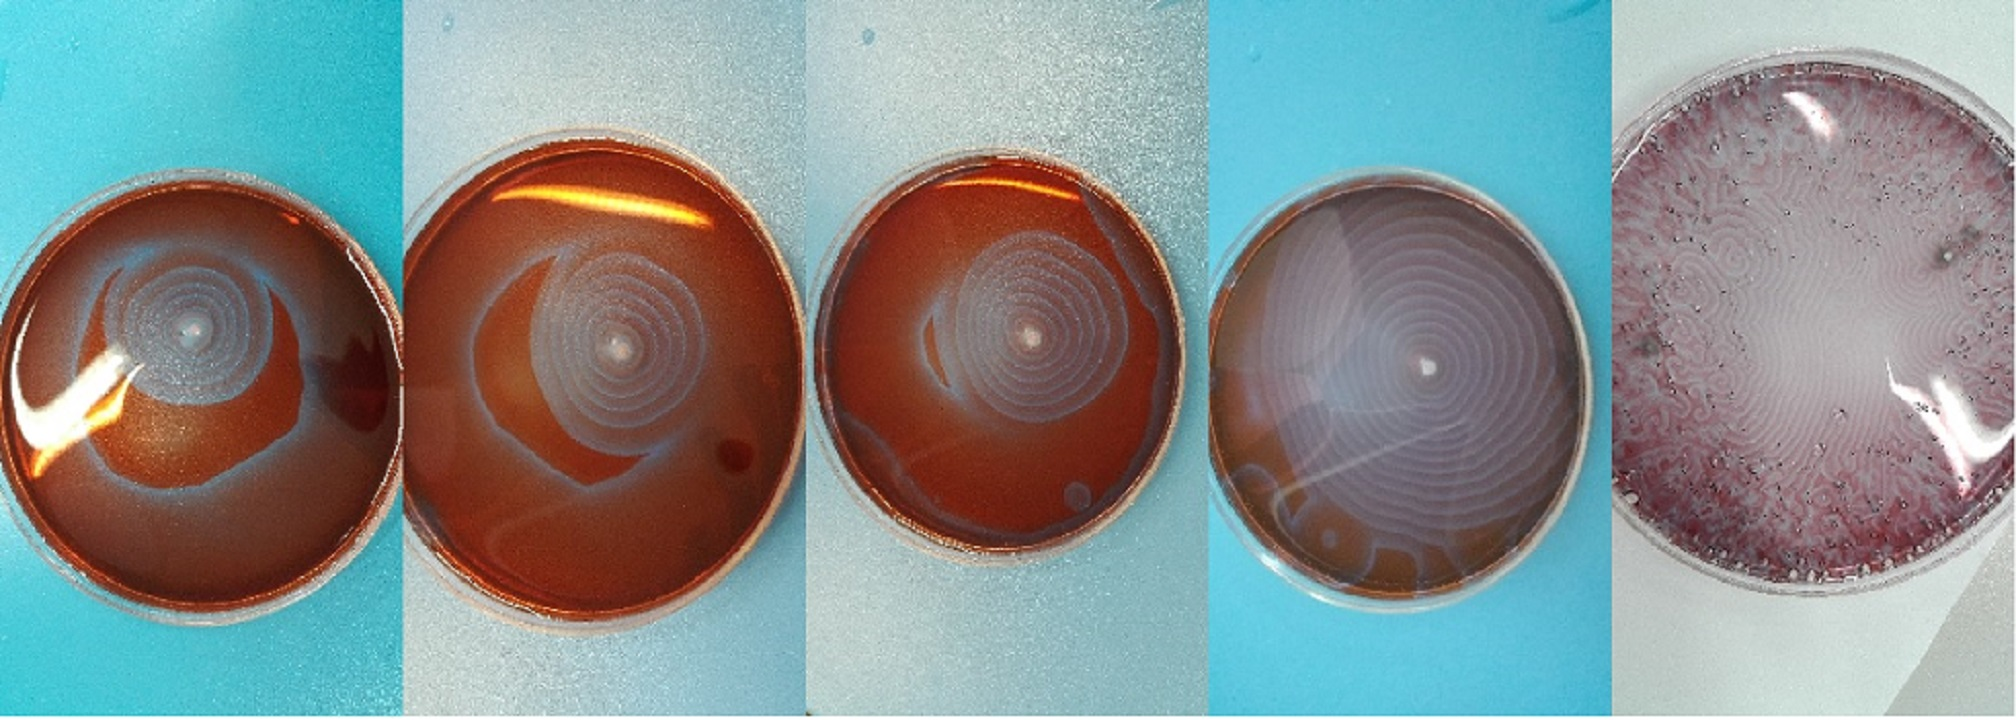
\includegraphics[width=0.8\textwidth]{img/oscillating_reaction.jpg}
\caption{BZ reakció Petri-csészében}
\label{fig:ionophores}
\end{figure}

Ezek a mintázatok dinamikus vagy stacionárius formában jelenhetnek meg.
Dinamikus formai megjelenés a mozgó kémiai hullámok, amelyek az idő előrehaladtával növekvő sugarú koncentrikus köröket képeznek, melyeket megzavarva jobbra- vagy balra forgó spirálok alakulhatnak ki.
Stacionárius térbeni szerkezetek esetében állóhullámok jelenhetnek meg, ilyen például a Turing struktúra, ami labirintus formájú sávok, vagy szabályos pontok térbeli mintázata.

